%%% Ne pas modifier jusqu'à la ligne 25
\documentclass[a4paper,12pt]{book}
\usepackage[utf8]{inputenc}
\usepackage[french]{babel}
%%\usepackage{CJK}
\usepackage{yhmath}
\usepackage[left=2cm,right=2cm,top=3cm,bottom=2cm, headheight=1.5cm,headsep=1.5cm]{geometry}
%%\usepackage{CJKutf8}
\usepackage{amsfonts}
\usepackage{amsmath,amsfonts,amssymb,dsfont}
\usepackage{graphicx}
\usepackage{enumitem}		%\enumerate-resume
\usepackage[colorlinks=true,unicode={true},hyperindex=false, linkcolor=blue, urlcolor=blue]{hyperref}
\newcommand{\myref}[1]{\ref{#1} page \pageref{#1}}

\addto\captionsfrench{\def\tablename{Tableau}}  %légendes des tableaux
\renewcommand\thesection{\Roman{section}~-~} 
\renewcommand\thesubsection{\Roman{section}.\Alph{subsection}~-~} 
\renewcommand\thesubsubsection{\Roman{section}.\Alph{subsection}.\arabic{subsubsection}~-~} 

\newcommand{\conclusion}[1]{\newline \centerline{\fbox{#1}}}

\setcounter{secnumdepth}{3}
\parindent=0pt

\usepackage{fancyhdr}
\pagestyle{fancy}

\lhead{SJTU-ParisTech} 
%%%%%%%%%%%%%%%%%%%%%%%%%%%%%%%%%%
\chead{DM9}
\rhead{Daniel 518261910024}

\begin{document}
\renewcommand{\labelitemi}{$\blacktriangleright$}
\renewcommand{\labelitemii}{$\bullet$}


\section{Exercice 1 : Saponification d’un ester}
\begin{table}[h]
\begin{center}
    \begin{tabular}{l|ccccccc}
    \hline
                      & $RCOOR^{'}$      & + & $HO^{-}$       & = & $RCOO^{-}$ & + & $R^{'}OH$ \\ \hline
        $c_{initial}(mol\,L^{-1})$ & $c_{1,i}=1.0*10^{-2}$       &   & $c_{2,i}=1.0*10^{-2}$      &   & $0$ &  & $0$\\ 
        $c_{final}(mol\,L^{-1})$      & $c_{1,f}=1.0*10^{-2}-\xi_v$  &   & $c_{2,f}=1.0*10^{-2}-\xi_v$  &   & $\xi_v$ & & $\xi_v$\\ 
    \end{tabular}
\end{center}
\end{table}
\subsection{}
En posant $c=c_{1,i}=c_{2,i}=1.0*10^{-2}\,mol\cdot L^{-1}$, on a 
$$v = k[RCOOR^{'}][HO^{-}]=\frac{d[R^{'}OH]}{dt}$$
d'où $k(c-\xi_v)^2=\frac{d\xi_v}{dt}$

\hspace*{\fill} 

Donc 
$$
\frac{-1}{\xi_v-c}-\frac{1}{c}=kt
$$
Donc $\boxed{x=\xi_v=c-\frac{1}{kt+\frac{1}{c}}}$
\subsection{}
On a au bout de $t=2h$, $\frac{c_{2,f}}{c_{2,i}}=25\%$, donc $\xi_v=\frac{3}{4}c$, on a donc $\frac{3}{4}c=c-\frac{1}{kt+\frac{1}{c}}$.

\hspace*{\fill} 

Donc, $\boxed{k=\frac{3}{ct}}$. A.N. $k=\frac{3}{1.0*10^{-2}*2*3600}=0.042\,mol\cdot L^{-1}$

\hspace*{\fill} 

la demi-réaction $t_{1/2}$ est définie par $\frac{[HO^{-}](t_{1/2})}{c}=0.5$, donc $\xi_v^{'}=\frac{1}{2}c$. 

\hspace*{\fill} 

On obtient $\boxed{t_{1/2}=\frac{1}{kc}}$. A.N. $\boxed{t_{1/2}=\frac{1}{1.0*10^{-2}*0.042}=2.4*10^3\,s}$, soit $40\,min$
\section{Exercice 2 : Substitution nucléophile}
\begin{table}[h]
    \begin{center}
        \begin{tabular}{l|ccccccc}
        \hline
                          & $RBr$      & + & $HO^{-}$       & = & $ROH$ & + & $Br^{-}$ \\ \hline
            $c_{initial}(mol\,L^{-1})$ & $c_{1,i}=0.010$       &   & $c_{2,i}=1.0$      &   & $0$ &  & $0$\\ 
            $c_{final}(mol\,L^{-1})$      & $c_{1,f}=0.010-\xi_v$  &   & $c_{2,f}=1.0-\xi_v$  &   & $\xi_v$ & & $\xi_v$\\ 
        \end{tabular}
    \end{center}
    \end{table}
\subsection{}
On va chercher à déterminer l’ordre de $RBr$, car $HO^{-}$ est en large excès.

\hspace*{\fill} 

Donc $[HO^{-}]_t\simeq [HO^{-}]_0$ au cours de cette réaction

\hspace*{\fill} 

Donc $\boxed{k_{app,1}=k[OH^{-}]_{0,1}}$, $v=k_{app,1}[RBr]$
\begin{figure}[h]
    \begin{center}
    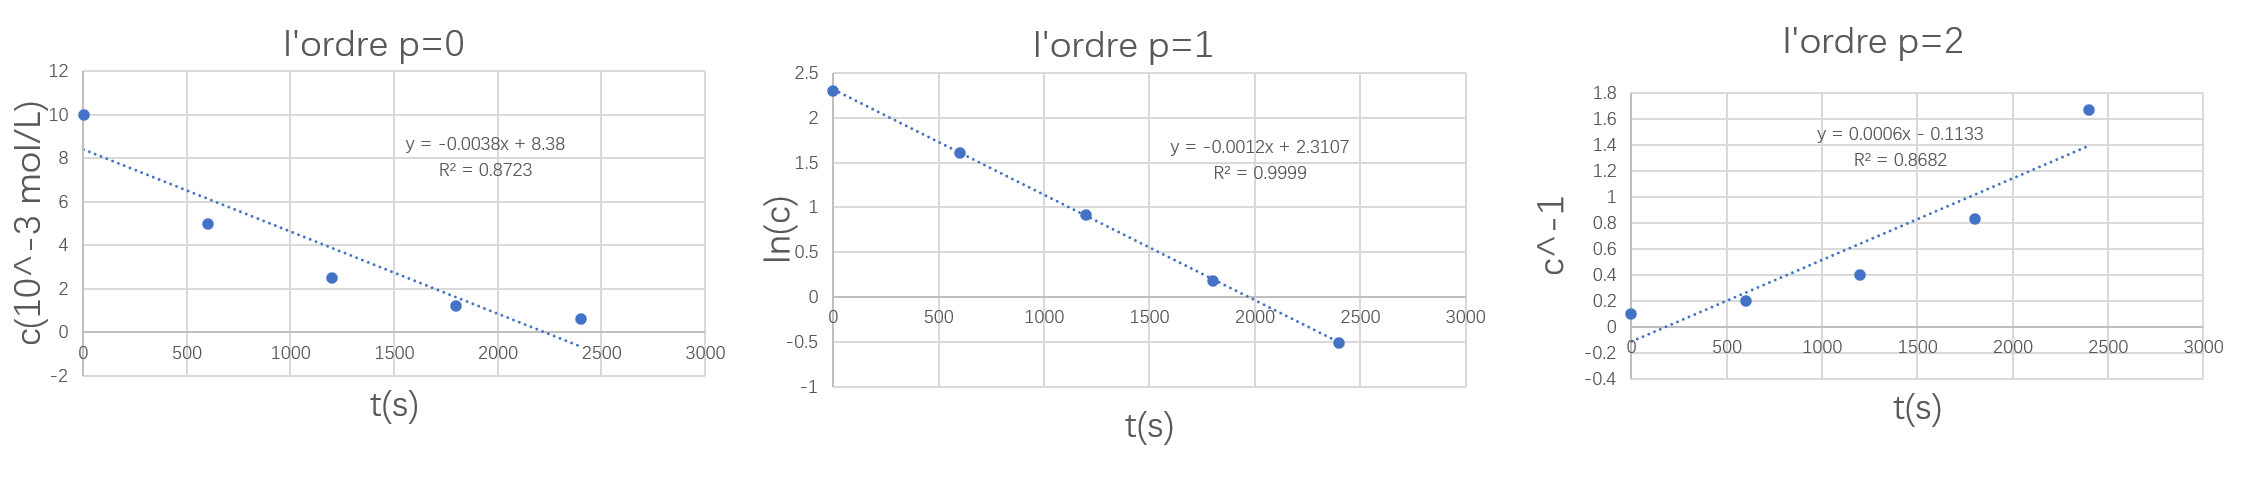
\includegraphics[scale=0.45]{dm91.png}
    \end{center}
    \caption{Ajustement de courbe}
\end{figure}

\hspace*{\fill} 

Par ajustement du courbe, on en déduit que cette réaction est d'ordre 1 par rapport à $RBr$

\hspace*{\fill} 

Sa pente $\boxed{k_{app,1}=-1*(-0.0012)=1.2*10^{-3}\,s^{-1}}$, donc $k=\frac{k_{app,1}}{[OH^{-}]_{0,1}}=1.2*10^{-3}\,L\cdot mol^{-1}\cdot s^{-1}$
\subsection{}
\begin{figure}[h]
    \begin{center}
    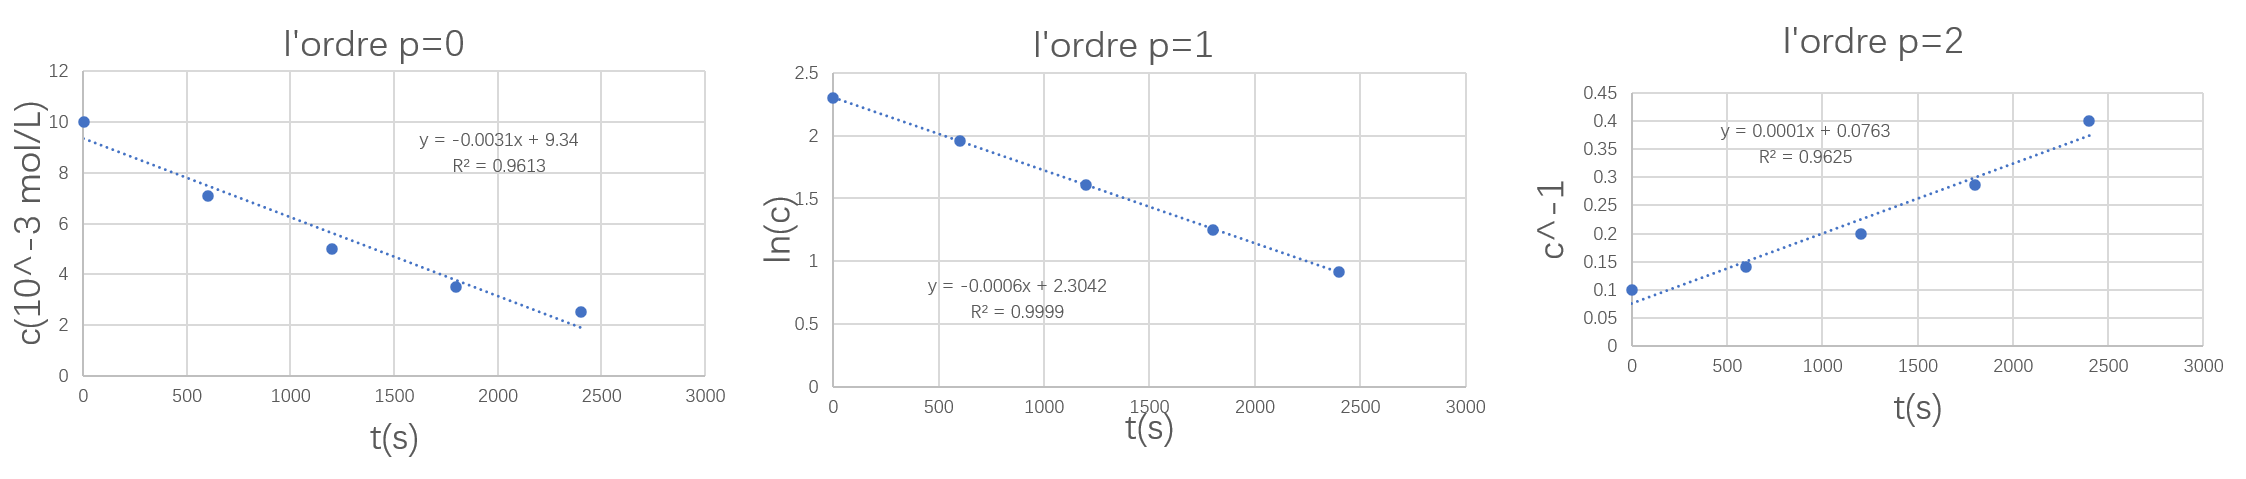
\includegraphics[scale=0.45]{dm92.png}
    \end{center}
    \caption{Ajustement de courbe}
\end{figure}
De la même méthode, si on suppose que $v=k_{app,2}[HBr]$, avec $k_{app,2}=k[OH^{-}]_{0,2}$

\hspace*{\fill} 

Par ajustement du courbe, on en déduit que cette réaction est d'ordre 1 par rapport à $RBr$

\hspace*{\fill} 

Sa pente $\boxed{k_{app,2}=-1*(-0.0006)=0.6*10^{-3}\,s^{-1}}$, donc $k=\frac{k_{app,2}}{[OH^{-}]_{0,2}}=1.2*10^{-3}\,L\cdot mol^{-1}\cdot s^{-1}$

\hspace*{\fill} 

$k_{app}$ est proportionnel à $[OH^{-}]$(supposé constante au cours de la réaction), on en déduit que la loi de vitesse $\boxed{v=k[OH^{-}][HBr]}$, 
où $[HBr]=[HBr]_0*e^{-k_{app}t}$, avec $k=1.2*10^{-3}\,L\cdot mol^{-1}\cdot s^{-1}$, $k_{app}=k[OH^{-}]$


\subsection{}
La transformation chimique peut s’expliquer par $S_N2$
\end{document}